\section{Definition of XBWT}
The \textbf{Extended Burrows-Wheeler Transform} is a data structure designed to efficiently compress and index \emph{labeled trees}. Inspired by the classical Burrows-Wheeler Transform (BWT) \cite{burrows1994block} for strings, the XBWT extends these principles to hierarchical structures, enabling efficient storage, navigation, and querying of trees. It is particularly effective for trees where each node has a label drawn from an alphabet $\Sigma$ and the tree structure has an arbitrary shape and degree.

Given an ordered labeled tree $T$ of arbitrary fan-out, depth and shape, with $n$ internal nodes and $l$ leaves ($t$ nodes in total) and alphabet $\Sigma$. Let $u$ be a node in $T$, we define the following information:
\begin{itemize}
    \item $last[u]$: is a binary value that is 1 if $u$ is the last (rightmost) child of its parent, and 0 otherwise.
    \item $\alpha[u]$: denotes the label of node $u$ plus one bit that is 1 if $u$ is a leaf and 0 otherwise.
    \item $\pi(u)$: is the string obtained by concatenating the labels of the nodes on the path from $u$'s parent to the root of $T$ (the root has an empty $\pi$ component).
\end{itemize}

Then, to define the XBWT, a sorted multi-set $S$ consisting of $t$ triplets (one per node of $T$) is built, where each triplet is of the form $(last[u], \alpha[u], \pi(u))$ for some node $u$ in $T$. $S$ is built by traversing $T$ in a pre-order fashion, for each visited node $u$, the triplet $(last[u], \alpha[u], \pi(u))$ is added to $S$, then $S$ is stably sorted in accordance with the lexicographic order of the $\pi$ component of the triplets.

\begin{theorem}
    The XBWT of a labeled tree $T$ consist of the two arrays $\{S_{\text{last}}, S_{\alpha}\}$ after sorting, and takes $2t + t \log |\Sigma|$ bits of space. 
\end{theorem}

\section{Properties of XBWT}
The following two properties of the ordered multi-set $S$ are crucial for the indexing scheme, they immediately follow from the composition of the transform and from the way $S$ is built.

\subsection{Property 1} \label{prop1}
\begin{enumerate}
    \item $S_{\text{last}}$ has $n$ 1s (one for each internal node) and $l$ 0s (one for each leaf).
    \item $S_{\alpha}$ is a permutation of the labels of the nodes in $T$.
    \item $S_{\pi}$ contains all the upward labeled paths of $T$ consisting internal node labels only. Also, each path is repeated a number of times equal to the number of its offsprings.
\end{enumerate}

\subsection{Property 2} \label{prop2}
\begin{enumerate}
    \item The first triplet of $S$ refers to the root of $T$.
    \item The triplet of node $u$ precedes the triplet of node $v$ in $S$ iff either $\pi[u] < \pi[v]$ or $\pi[u] = \pi[v]$ and $u$ precedes $v$ in the pre-order traversal of $T$.
    \item Let $u_1, \dots, u_z$ be the children of node $u$ in $T$, then the triplets of $u_1, \dots, u_z$ are consecutive in $S$ following this order. Moreover, the subarray $S_{\text{last}}[u_1 \dots u_z]$ provides the unary encoding of $u$'s degree, namely $S_{\text{last}}[u_z] = 1$ and $S_{\text{last}}[u_i] = 0$ for $1 \leq i < z$.
    \item Let $u, v$ be two nodes in $T$ having the same label $\alpha[u] = \alpha[v]$, then if the triplets of $u$ precedes the triplets of $v$ in $S$, then the contiguous block of children of $u$ in $S$ precedes the contiguous block of children of $v$ in $S$. 
\end{enumerate}

\subsection{Property 3} \label{prop3}
Let $c \in \Sigma$ be an internal node label, and let $S[j_1, j_2]$ be all triplets whose $\pi$-components are prefixed by $c$. If $u$ is the $i$-th node labeled $c$ in $S_{\alpha}$, its children occur contiguously within $S[j_1, j_2]$ and delimited by the $i - 1$-th and $i$-th bit set to 1 in $S_{\text{last}}[j_1, j_2]$.

\section{XBWT Construction}
A naive approach to build the XBWT would be to explicitly construct $S$ through the concretization of $\pi$-strings and then sort it using a stable sorting algorithm. However, this approach would require $\Theta(t^2)$ space in the worst case, which is not feasible for large deep trees. To overcome this issue, Ferragina et al. \cite{ferragina2009compressing} proposed a more efficient algorithm that builds $S$ in linear time and $O(t \log t)$ space.

The linear time algorithm is called \textbf{pathSort}, it is based on a generalization of the Skew algorithm for suffix array construction of strings \cite{karkkainen2006linear}. Let's see briefly how the Skew algorithm works.

\begin{figure}
    \centering
    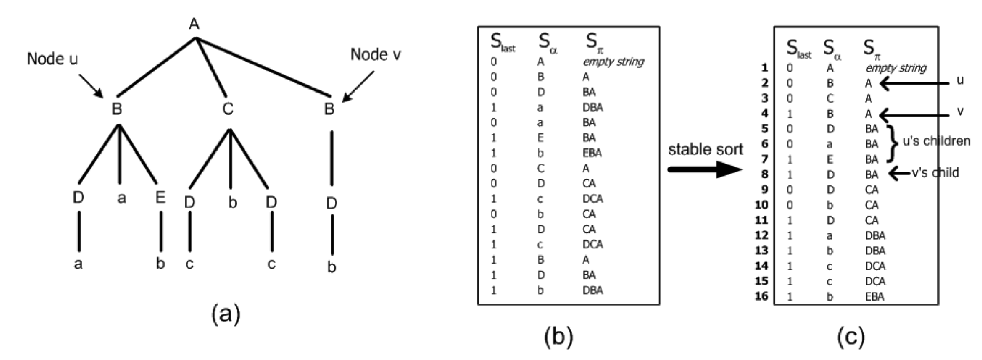
\includegraphics[width=1\textwidth]{Immagini/XBWT_example.png}
    \caption[XBWT example]{(a) A labeled tree $T$ where $\Sigma_N = \{A, B, C, D, E\}$ and $\Sigma_L = \{a, b, c\}$. Notice that $\alpha[u] = \alpha[v] = B$ and $\pi[u] = \pi[v] = A$. (b) The multi-set $S$ obtained after the pre-order visit of $T$. (c) The final multi-set $S$ after the stable sort based on the $\pi$'s component of its triplets.}
    \label{fig:XBWT_example}
\end{figure}

\subsection{Skew Algorithm}
The Skew algorithm is an efficient method for constructing the suffix array of a string in linear time. A suffix array is a data structure that lists the starting indices of all the suffixes of a string in lexicographical order, and it is widely used in various string processing algorithms.

\subsubsection*{Algorithm Overview}

\subsubsection*{1. Divide the String}

The algorithm begins by partitioning the indices of the string into three groups based on their modulo 3 value:
\begin{itemize}
    \item $S_0$: Indices congruent to 0 mod 3.
    \item $S_1$: Indices congruent to 1 mod 3.
    \item $S_2$: Indices congruent to 2 mod 3.
\end{itemize}

The suffixes starting at positions in $S_1$ and $S_2$ are combined into a single group called $S_{12}$.

\subsubsection*{2. Sort Suffixes in $S_{12}$}

To sort the suffixes in $S_{12}$, the algorithm considers the triplets of characters starting at each position in $S_{12}$. These triplets are sorted using a linear-time sorting algorithm, such as radix sort, and then renamed by assigning each triplet an integer value representing its rank in the sorted order. If all triplets are unique, the sorting is complete; otherwise, the same procedure is applied recursively to the sequence of ranks obtained.

\subsubsection*{3. Sort Suffixes in $S_0$}

Once the suffixes in $S_{12}$ are sorted, the algorithm proceeds to sort the suffixes in $S_0$. To compare two suffixes starting at positions $i$ and $j$ in $S_0$, it compares the first characters of their respective substrings. If these are equal, it compares the suffixes starting at positions $i+1$ and $j+1$, whose ranks are already known from the sorting of $S_{12}$.

\subsubsection*{4. Merge the Sorted Orders}

Finally, the sorted orders of the suffixes in $S_0$ and $S_{12}$ are merged to obtain the complete suffix array of the original string. This merging process can be performed in linear time, ensuring the overall efficiency of the algorithm.

\subsection{PathSort Algorithm}

The pseudocode of the pathSort algorithm is shown in Algorithm \ref{alg:pathSort}. As we can see the algorithm is based on the Skew algorithm, but it is adapted to work on labeled trees. The main idea is to recursively sort the upward subpaths of the tree starting at nodes in levels $\not\equiv j \pmod{3}$, then sort the upward subpaths starting at nodes in levels $\equiv j \pmod{3}$ using the result of the previous step, and finally merge the two sets of sorted subpaths by exploiting their lexicographic names. The value of $j$ is chosen in such a way that the number of nodes in \texttt{IntNodes} whose level is $\equiv j \pmod{3}$ is at least $t/3$ so that a constant fraction of upward paths are ensured to be dropped at each recursive step. Is important to note that:
\begin{enumerate}
    \item The height of the new (contracted) tree shrinks by a factor three, hence the node naming requires the radix sort over triples of names; 
    \item given the choice of $j$, the number of nodes of the new (contracted) tree will be at most $2t/3$, thus ensuring that the running time of the algorithm satisfies the recurrence $R(t) = R(2t/3) + \Theta(t) = \Theta(t)$; 
    \item following an argument similar to \cite{karkkainen2006linear}, the names of the dropped subpaths can be computed in $O(t)$ time from the names of the non dropped subpaths, by radix sorting.
\end{enumerate}

\begin{algorithm}
    \caption{\textsc{PathSort}($T$)}
    \label{alg:pathSort}
    \begin{algorithmic}[1]
    \State Create the array \texttt{IntNodes}[1, $t$], initially empty.
    \State Visit the internal nodes of $T$ in pre-order. Let $u$ denote the $i$-th visited node.
    \State Write in \texttt{IntNodes}[$i$] the symbol $\alpha[u]$, the level of $u$ in $T$, and the position in \texttt{IntNodes} of $u$'s parent.
    \State Let $j \in \{0, 1, 2\}$ be such that the number of nodes in \texttt{IntNodes} whose level is $\equiv j \pmod{3}$ is at least $t/3$. Sort recursively the upward subpaths starting at nodes in levels $\not\equiv j \pmod{3}$.
    \State Sort the upward subpaths starting at nodes in levels $\equiv j \pmod{3}$ using the result of Step 3.
    \State Merge the two sets of sorted subpaths by exploiting their lexicographic names.
    \end{algorithmic}
\end{algorithm}

\subsubsection{Recursive Step of PathSort}
At each recursive step, the algorithm constructs the array \texttt{IntNodes} (as shown in Figure \ref{fig:XBWT_example}-(b)), which stores the triplets $(\alpha[u], \text{level}(u), \text{parent}(u))$ for every internal node $u$ in the given tree $T$.  

Next, the algorithm selects a value $j$ such that the number of nodes in \texttt{IntNodes} with depth $\equiv j \pmod{3}$ is at least $t/3$. Based on this choice, two separate arrays are created:  
\begin{itemize}
    \item \texttt{IntNodesAtPosJ}, containing nodes at levels $\equiv j \pmod{3}$,
    \item \texttt{IntNodesNotAtPosJ}, containing nodes at levels $\not\equiv j \pmod{3}$
\end{itemize}

For each node $u$ in \texttt{IntNodesNotAtPosJ}, the algorithm extracts the upward path consisting of the first three ancestors of $u$. These paths are then sorted using radix sort. If the sorted upward paths contain duplicates, the algorithm recursively calls the PathSort function on a new contracted tree, where nodes are renamed according to their sorted paths. Otherwise, if all upward paths are unique, the nodes in \texttt{IntNodesAtPosJ} are sorted and subsequently merged with \texttt{IntNodesNotAtPosJ} using lexicographic ordering, following the same merging strategy as in the Skew algorithm.

\section{Inverting the XBWT}
Property 3 \ref{prop3} ensures that the two array $S_{\text{last}}$ and $S_{\alpha}$ of the XBWT can be used to reconstruct the original tree $T$. The algorithm to invert the XBWT is linear in time and requires $O(t \log t)$ bits of space.

The algorithm \ref{alg:rebuildTree} initially builds the array $F$ that stores the first entry in $S$ whose $\pi$-component is prefixed by a symbol $x$ ($F$ approximates $S_{\pi}$ at its first symbol). Then, it exploits the array $F$ to efficiently build the array $J$ that stores the position in $S$ of the first child of each node in $T$. Finally, the algorithm deploys the array $J$ to
simulate a depth-first visit of $T$, creates its labeled nodes, and properly connects them to their parents. 

\begin{algorithm}[H]
    \caption{RebuildTree(\texttt{xbw[$T$]})}
    \label{alg:rebuildTree}
    \begin{algorithmic}[1]
    \State $F = $ BuildF(\texttt{xbw[$T$]}); \Comment{$F[x]$ = first entry in $S$ whose $\pi$-component is prefixed by symbol $x$}
    \State $J = $ BuildJ(\texttt{xbw[$T$]}, $F$); \Comment{$J[i]$ = position in $S$ of the first child of $S[i]$; $J[i] = -1$ if leaf}
    \State Create node $r$ and set $Q = \{(1, r)\}$; \Comment{$Q$ is a stack}
    \While{$Q \neq \emptyset$} \Comment{We still have nodes to create in $T$}
        \State $\langle i, u \rangle = $ pop($Q$);
        \State $j = J[i]$; \Comment{Take the block of $u$'s children in $S$}
        \If{$j = -1$} \Comment{$u$ is a leaf of $T$}
            \State \textbf{continue};
        \EndIf
        \State Find first $j' \geq j$ such that $S_{\text{last}}[j'] = 1$; \Comment{$S[j, j']$ are the children of $u$ in $T$}
        \For{$h = j'$ downto $j$} \Comment{Recall that $Q$ is a stack}
            \State Create the node $v$ labeled $S_\alpha[h]$;
            \State Attach $v$ as first child of $u$;
            \State push($\langle h, v \rangle$, $Q$);
        \EndFor
    \EndWhile
    \State \Return node $r$.
    \end{algorithmic}
\end{algorithm}

\begin{algorithm}[H]
    \caption{BuildF(\texttt{xbw[$T$]})}
    \label{alg:buildF}
    \begin{algorithmic}[1]
    \For{$i = 1, \ldots, |\Sigma_N|$}
        \State $C[S_\alpha[i]] \gets C[S_\alpha[i]] + 1$; \Comment{Count the occurrences of node labels}
    \EndFor
    \State $F[1] = 2$; \Comment{$S_\pi[1]$ is the empty string}
    \For{$i = 1, \ldots, |\Sigma_N| - 1$} \Comment{Consider just the internal-node labels}
        \State $s = 0$; $j = F[i]$;
        \While{$s \neq C[i]$} \Comment{Not all blocks of children have been passed}
            \If{$S_{\text{last}}[j++] = 1$} $s++$; \Comment{One further block of children has passed}
            \EndIf
        \EndWhile
        \State $F[i+1] = j$;
    \EndFor
    \State \Return $F$.
    \end{algorithmic}
\end{algorithm}
    
\begin{algorithm}[H]
    \caption{BuildJ(\texttt{xbw[$T$]}, $F$)}
    \begin{algorithmic}[1]
    \For{$i = 1, \ldots, t$}
        \If{$S_\alpha[i] \in \Sigma_L$}
            \State $J[i] = -1$; \Comment{$S_\alpha[i]$ is a leaf label}
        \Else
            \State $z = J[S_\alpha[i]]$;
            \While{$S_{\text{last}}[z] \neq 1$} $z++$; \Comment{Reach the last child of $S_\alpha[i]$}
            \EndWhile
            \State $F[S_\alpha[i]] = z + 1$;
        \EndIf
    \EndFor
    \State \Return $J$.
    \end{algorithmic}
\end{algorithm}

\section{Compressing Labeled Trees}
Let the $k$-context of a node $u$ in a tree $T$ be defined as the first $k$ symbols of the $\pi$-component of the triplet associated with $u$. We denote this $k$-long prefix as $\pi_k[u]$. Thus, $\pi_k[u]$ represents the subpath of length $k$ leading to $u$ in $T$, or equivalently, the node $u$ descends from a subpath labeled as $\pi_k[u]$, where the nodes in $\pi_k[u]$ are encountered in an upward direction.

The XBW[$T$] exhibits a local homogeneity property on the string $S_{\alpha}$, which can be demonstrated through the concept of $k$-contexts on trees. This property mirrors the strong local homogeneity exhibited by strings under the Burrows-Wheeler Transform [Burrows and Wheeler 1994] when applied to labeled trees. Specifically, node labels in $T$ are distributed across $S_{\alpha}$ in a manner that clusters together those labels originating from "similar" upward paths that share long prefixes. 

To illustrate this, let us consider two arbitrary nodes $u$ and $v$ in $T$, and examine their contexts $\pi[u]$ and $\pi[v]$. Given the sorting of $S$, the greater the length of the shared prefix between $\pi[u]$ and $\pi[v]$, the closer the corresponding labels $\alpha[u]$ and $\alpha[v]$ will be in the string $S_{\alpha}$. These closely spaced labels are expected to be few in number, resulting in $S_{\alpha}$ exhibiting local homogeneity. As a consequence, we can leverage the advanced algorithmic techniques developed for BWT-based compression methods to achieve efficient compression.

At the end, the XBWT is used for turning the labeled tree compression problem into a string compression problem. To this aim, two string compressors
$C_{\alpha}$ and $C_{\text{last}}$ are used to squeeze the two strings that compose XBW[$T$], by exploiting their fine specialties. Of course, many choices are possible for $C_{\text{last}}$ and $C_{\alpha}$, each having implications on the algorithmic time and compression bounds.

In general, let $C_{\alpha}$ be a $k$-th order string compressor that compresses any string $w$ into $|w|H_k(w) + |w| + o(|w|)$ bits, taking $O(|w|)$ time; and let $C_{\text{last}}$ be an algorithm that stores $S_{\text{last}}$ without compression. With this simple instantiation, the labeled tree $T$ can be compressed within $t H_k(S_{\alpha}) + 2t + o(t)$ bits and takes $O(t)$ optimal time.

\section{Indexing a compressed labeled tree}
In order to implement the efficient operations listed in \ref{compandindexinglabtree} using the compressed arrays $S_{\text{last}}$ and $S_{\alpha}$ of XBWT, we need that the chosen compressors $C_{\alpha}$ and $C_{\text{last}}$ support the following operations:

Given a string $S[1, t]$ over alphabet $\Sigma$
\begin{itemize}
    \item \textbf{$rank_c(S, q)$}: gives the number of times the symbol $c \in \Sigma$ appears in $S[1, q]$.
    \item \textbf{$select_c(S, i)$}: gives the position of the $i$-th occurrence of the symbol $c \in \Sigma$ in $S$.
\end{itemize}

The compressed indexing of XBWT[$T$] will be based on three compressed data structures that support rank and select queries over the two strings $S_{\alpha}$ and $S_{\text{last}}$, and over an auxiliary binary array $A[1, t]$ defined as: $A[1] = 1$, $A[j] = 1$ if and only if the first symbol of $S_{\pi}[j]$ differs from the first symbol of $S_{\pi}[j - 1]$. Hence, $A$ contains at most $|\Sigma| + 1$ bits set to 1 out of $t$ positions. It is also easy to see that, by means of rank and select operations over $A$, we can succinctly implement the array $F$ deployed in the algorithms \ref{alg:rebuildTree} and \ref{alg:buildF}.

The following methods are supported by the compressed index:
\begin{itemize}
    \item \textbf{GetRankedChild(i, k)}: returns the position in $S$ of the $k$-th child of $u$; the output is $-1$ if this child does not exist. As an example, \texttt{GetRankedChild(2, 2) = 6} in Figure \ref{fig:XBWT_example}.
    \item \textbf{GetCharRankedChild(i, c, k)}: returns the position in $S$ of the triplet representing the $k$-th child of $u$ among the ones whose label is $c$. The output is $-1$ if this child does not exist. As an example, \texttt{GetCharRankedChild(1, B, 2) = 4} in Figure \ref{fig:XBWT_example}.
    \item \textbf{GetDegree(i)}: returns the number of children of $u$.
    \item \textbf{GetCharDegree(i, c)}: returns the number of children of $u$ labeled $c$.
    \item \textbf{GetParent(i)}: returns the position in $S$ of the triplet representing the parent of $u$. The output is $-1$ if $i = 1$ (the root). As an example, \texttt{GetParent(8) = 4} in Figure \ref{fig:XBWT_example}.
    \item \textbf{GetSubtree(i)}: returns the node labels of the subtree rooted at $u$. Any possible order (i.e., pre, in, post) may be implemented.
    \item \textbf{SubPathSearch($P$)}: determines the range $S[\text{First}, \text{Last}]$ of nodes, which are immediate descendants of each occurrence of the labeled path $P = c_1c_2 \cdots c_k$ in $T$. Note that all strings in $S_{\pi}[\text{First}, \text{Last}]$ are prefixed by $P^R$. As an example, \texttt{SubPathSearch(BD) = [12, 13]} and \texttt{SubPathSearch(AB) = [5, 8]} in Figure \ref{fig:XBWT_example}.
\end{itemize}

It is important to note that their time complexity is dependent on the specific implementation for rank and select over the compressed strings $S_{\alpha}$ and $S_{\text{last}}$. 

Let's now see how to implement some of the above methods (from which the others can be derived) using the rank and select operations over the compressed strings $S_{\alpha}$ and $S_{\text{last}}$.

\subsubsection*{GetChildren(i)}

\begin{algorithm}[H]
    \caption{GetChildren($i$)}
    \begin{algorithmic}[1]
    \If{$S_\alpha[i] \in \Sigma_L$}
        \State \Return $-1$ \Comment{$S[i]$ is a leaf}
    \EndIf
    \State $c \gets S_\alpha[i]$ \Comment{$S[i]$ is labeled $c$}
    \State $r \gets \text{rank}_c(S_\alpha, i)$
    \State $y \gets \text{select}_1(A, c)$ \Comment{$y = F[c]$}
    \State $z \gets \text{rank}_1(S_{\text{last}}, y - 1)$
    \State $\text{First} \gets \text{select}_1(S_{\text{last}}, z + r - 1) + 1$
    \State $\text{Last} \gets \text{select}_1(S_{\text{last}}, z + r)$
    \State \Return $(\text{First}, \text{Last})$
    \end{algorithmic}
\end{algorithm}

The algorithm exploits directly the properties described before, in particular the Property 3 (\ref{prop3}). The rank operation at line 5 is used to get the number $r$ of nodes labeled $c$ up to position $i$ in $S_{\alpha}$. Then, the position $F[c] $through a select operation on $A$ (line 6). By Property 3, the children of $S[i]$ are located at the $r$-th block of children following position $F[c]$. Lines $8 - 9$ identify this block. 

\subsubsection*{GetParent(i)}

\begin{algorithm}[H]
    \caption{GetParent($i$)}
    \label{alg:getparent}
    \begin{algorithmic}[1]
    \If{$i == 1$}
        \State \Return $-1$ \Comment{$S[i]$ is the root of $\mathcal{T}$}
    \EndIf
    \State $c \gets \text{rank}_1(A, i)$
    \State $y \gets \text{select}_1(A, c)$
    \State $k \gets \text{rank}_1(S_{\text{last}}, i - 1) - \text{rank}_1(S_{\text{last}}, y - 1)$
    \State $p \gets \text{select}_c(S_\alpha, k + 1)$
    \State \Return $p$
    \end{algorithmic}
\end{algorithm}

Algorithm \ref{alg:getparent} is based on the Property 3 (\ref{prop3}) and it is the inverse of the GetChildren method. At line 4 the algorithm computes the label $c$ of the parent of $S[i]$ that prefixes the upward path leading to $S[i]$. Then, the parent of $S[i]$ is searched among the nodes labeled $c$ in $S_{\alpha}$ by exploiting Property 3 in a reverse manner. Namely, the number $k$ of children-blocks in the range $S[y, i]$ is computed, these are children of nodes labeled $c$ and preceding $i$ in the stable sort of $S$. Then, the $k$-th occurrence of $c$ in $S_{\alpha}$ is selected, which is properly the parent of $S[i]$.

\subsubsection*{SubPathSearch($P$)}

\begin{algorithm}[H]
    \caption{SubPathSearch($P$)}
    \label{alg:subpathsearch}
    \begin{algorithmic}[1]
    \State $First \gets F(c_1)$; $Last \gets F(c_1 + 1) - 1$
    \If{$First > Last$}
        \State \textbf{return} ``$P$ is not a subpath of $T$''
    \EndIf
    \For{$i \gets 2, \dots, k$}
        \State $k_1 \gets \text{rank}_{c_i}(S_\alpha, First - 1)$; $z_1 \gets \text{select}_{c_i}(S_\alpha, k_1 + 1)$
        \Comment{first entry in $S_\alpha[First, t]$ labeled $c_i$}
        \State $k_2 \gets \text{rank}_{c_i}(S_\alpha, Last)$; $z_2 \gets \text{select}_{c_i}(S_\alpha, k_2)$
        \Comment{last entry in $S_\alpha[1, Last]$ labeled $c_i$}
        \If{$z_1 > z_2$}
            \State \textbf{return} ``$P$ is not a subpath of $T$''
        \EndIf
        \State $First \gets \text{GetRankedChild}(z_1, 1)$ \Comment{get the first child of $S[z_1]$}
        \State $Last \gets \text{GetRankedChild}(z_2, \text{GetDegree}(z_2))$ \Comment{get the last child of $S[z_2]$}
    \EndFor
    \State \textbf{return} $(First, Last)$
    \end{algorithmic}
\end{algorithm}

We assume that $P = c_1c_2 \cdots c_k$ algorithm SubPathSearch computes the range $[First, Last]$ in $|P| = l$ phases, each one preserving the following invariant:

\begin{itemize}
    \item Invariant of Phase $i$. At the end of the phase, $S_{\pi}[First]$ is the first entry prefixed by $P[1, i]^R$ , and $S_{\pi}[Last]$ is the last entry prefixed by $P[1, i]^R$ , where $s^R$ is the reversal of string $s$.
\end{itemize}

At the beginning (i.e., $i = 1$), First and Last are easily determined via the entries $F[c_1]$ and $F[c_1 + 1] - 1$, which point to the first and last entry of $S_{\pi}$ prefixed by $c_1$ (by definition of array $F$). Since we do not have the $F$ array, we implement these operations via rank and select queries over array $A$. Let us assume that the invariant holds for Phase $i - 1$, and prove that the $i$-th iteration of the for-loop in algorithm SubPathSearch preserves the invariant. More precisely, let $S_{\pi}[First, Last]$ be all entries prefixed by $P[1, i - 1]^R$. So $S[First, Last]$ contains all nodes descending from $P[1, i - 1]$. SubPathSearch determines $S[z_1]$ (respectively $S[z_2]$) as the first (respectively last) node in $S[First, Last]$ that descends from $P[1, i - 1]$ and is labeled $c_i$, if any. Then it jumps to the first child of $S[z_1]$ and the last child of $S[z_2]$. From Property 2 (item 2), and the correctness of algorithms GetChildren and GetDegree, we infer that the positions of these two children are exactly the first (respectively last) entry in $S$ whose $\pi$-component is prefixed by $P[1, i]^R$. 

The time complexity of the SubPathSearch algorithm is $O(l)$, where $l$ is the length of the input path $P$.
